%----------------------------------------------------------------------------------------
%	PACKAGES AND OTHER DOCUMENT CONFIGURATIONS
%----------------------------------------------------------------------------------------

\documentclass[
	11pt, % Set the default font size, options include: 8pt, 9pt, 10pt, 11pt, 12pt, 14pt, 17pt, 20pt
	%t, % Uncomment to vertically align all slide content to the top of the slide, rather than the default centered
	aspectratio=169, % Uncomment to set the aspect ratio to a 16:9 ratio which matches the aspect ratio of 1080p and 4K screens and projectors
]{beamer}

\graphicspath{{figures/}{./}} % Specifies where to look for included images (trailing slash required)

\usepackage{booktabs} % Allows the use of \toprule, \midrule and \bottomrule for better rules in tables
\usepackage{caption}
\usepackage{tikz}
\usepackage{amsmath}
\usepackage{amssymb}
\usepackage{placeins}
\usepackage{mathtools}
\usepackage{hyperref}

%----------------------------------------------------------------------------------------
%	SELECT LAYOUT THEME
%----------------------------------------------------------------------------------------

% Beamer comes with a number of default layout themes which change the colors and layouts of slides. Below is a list of all themes available, uncomment each in turn to see what they look like.

%\usetheme{default}
%\usetheme{AnnArbor}
%\usetheme{Antibes}
%\usetheme{Bergen}
%\usetheme{Berkeley}
%\usetheme{Berlin}
%\usetheme{Boadilla}
%\usetheme{CambridgeUS}
%\usetheme{Copenhagen}
%\usetheme{Darmstadt}
%\usetheme{Dresden}
%\usetheme{Frankfurt}
%\usetheme{Goettingen}
%\usetheme{Hannover}
%\usetheme{Ilmenau}
%\usetheme{JuanLesPins}
%\usetheme{Luebeck}
\usetheme{Madrid}
%\usetheme{Malmoe}
%\usetheme{Marburg}
%\usetheme{Montpellier}
%\usetheme{PaloAlto}
%\usetheme{Pittsburgh}
%\usetheme{Rochester}
%\usetheme{Singapore}
%\usetheme{Szeged}
%\usetheme{Warsaw}

%----------------------------------------------------------------------------------------
%	SELECT COLOR THEME
%----------------------------------------------------------------------------------------

% Beamer comes with a number of color themes that can be applied to any layout theme to change its colors. Uncomment each of these in turn to see how they change the colors of your selected layout theme.

%\usecolortheme{albatross}
%\usecolortheme{beaver}
%\usecolortheme{beetle}
%\usecolortheme{crane}
%\usecolortheme{dolphin}
%\usecolortheme{dove}
%\usecolortheme{fly}
% \usecolortheme{lily}
% \usecolortheme{monarca}
% \usecolortheme{seagull}
%\usecolortheme{seahorse}
%\usecolortheme{spruce}
% \usecolortheme{whale}
%\usecolortheme{wolverine}

%----------------------------------------------------------------------------------------
%	SELECT FONT THEME & FONTS
%----------------------------------------------------------------------------------------

% Beamer comes with several font themes to easily change the fonts used in various parts of the presentation. Review the comments beside each one to decide if you would like to use it. Note that additional options can be specified for several of these font themes, consult the beamer documentation for more information.

\usefonttheme{default} % Typeset using the default sans serif font
%\usefonttheme{serif} % Typeset using the default serif font (make sure a sans font isn't being set as the default font if you use this option!)
%\usefonttheme{structurebold} % Typeset important structure text (titles, headlines, footlines, sidebar, etc) in bold
%\usefonttheme{structureitalicserif} % Typeset important structure text (titles, headlines, footlines, sidebar, etc) in italic serif
%\usefonttheme{structuresmallcapsserif} % Typeset important structure text (titles, headlines, footlines, sidebar, etc) in small caps serif

%------------------------------------------------

%\usepackage{mathptmx} % Use the Times font for serif text

%\usepackage{helvet} % Use the Helvetica font for sans serif text
%\usepackage[default]{FiraSans} % Use the Fira Sans font for sans serif text
%\usepackage[default]{lato} % Use the Lato font for sans serif text

%----------------------------------------------------------------------------------------
%	SELECT INNER THEME
%----------------------------------------------------------------------------------------

% Inner themes change the styling of internal slide elements, for example: bullet points, blocks, bibliography entries, title pages, theorems, etc. Uncomment each theme in turn to see what changes it makes to your presentation.

%\useinnertheme{default}
\useinnertheme{circles}
%\useinnertheme{rectangles}
%\useinnertheme{rounded}
%\useinnertheme{inmargin}

%----------------------------------------------------------------------------------------
%	SELECT OUTER THEME
%----------------------------------------------------------------------------------------

% Outer themes change the overall layout of slides, such as: header and footer lines, sidebars and slide titles. Uncomment each theme in turn to see what changes it makes to your presentation.

%\useoutertheme{default}
%\useoutertheme{infolines}
%\useoutertheme{miniframes}
%\useoutertheme{smoothbars}
%\useoutertheme{sidebar}
%\useoutertheme{split}
%\useoutertheme{shadow}
%\useoutertheme{tree}
%\useoutertheme{smoothtree}

%\setbeamertemplate{footline} % Uncomment this line to remove the footer line in all slides
%\setbeamertemplate{footline}[page number] % Uncomment this line to replace the footer line in all slides with a simple slide count

%\setbeamertemplate{navigation symbols}{} % Uncomment this line to remove the navigation symbols from the bottom of all slides

%----------------------------------------------------------------------------------------
%	PRESENTATION INFORMATION
%----------------------------------------------------------------------------------------

\title[New Optimizer I]{New Optimizer I} % The short title in the optional parameter appears at the bottom of every slide, the full title in the main parameter is only on the title page

\subtitle{} % Presentation subtitle, remove this command if a subtitle isn't required

\author[]{Alexander Ludwig} % Presenter name(s), the optional parameter can contain a shortened version to appear on the bottom of every slide, while the main parameter will appear on the title slide


\date[\today]{Deep Learning Research Kitchen (ML-4501 / 3 ECTS) \\ \today} % Presentation date or conference/meeting name, the optional parameter can contain a shortened version to appear on the bottom of every slide, while the required parameter value is output to the title slide

%----------------------------------------------------------------------------------------

\AtBeginSection[]{
  \begin{frame}
  \vfill
  \centering
  \begin{beamercolorbox}[sep=8pt,center,shadow=true,rounded=true]{title}
    \usebeamerfont{title}\insertsectionhead\par%
  \end{beamercolorbox}
  \vfill
  \end{frame}
}

\begin{document}

%----------------------------------------------------------------------------------------
%	TITLE SLIDE
%----------------------------------------------------------------------------------------

\begin{frame}
	\titlepage % Output the title slide, automatically created using the text entered in the PRESENTATION INFORMATION block above
\end{frame}

%----------------------------------------------------------------------------------------
%	TABLE OF CONTENTS SLIDE
%----------------------------------------------------------------------------------------

% The table of contents outputs the sections and subsections that appear in your presentation, specified with the standard \section and \subsection commands. You may either display all sections and subsections on one slide with \tableofcontents, or display each section at a time on subsequent slides with \tableofcontents[pausesections]. The latter is useful if you want to step through each section and mention what you will discuss.

\begin{frame}
	\frametitle{Structure} % Slide title, remove this command for no title
	
	\tableofcontents % Output the table of contents (all sections on one slide)
	%\tableofcontents[pausesections] % Output the table of contents (break sections up across separate slides)
\end{frame}

%----------------------------------------------------------------------------------------
%	PRESENTATION BODY SLIDES
%----------------------------------------------------------------------------------------

\section{} % Sections are added in order to organize your presentation into discrete blocks, all sections and subsections are automatically output to the table of contents as an overview of the talk but NOT output in the presentation as separate slides

%------------------------------------------------

\subsection{New but famous optimizers}

\begin{frame}
	\frametitle{AdamW: decoupling weight decay from your adaptive optimizer}
	\framesubtitle{more state of the art research from Freiburg}
	 \begin{columns}[c] % The "c" option specifies centered vertical alignment while the "t" option is used for top vertical alignment
		\begin{column}{0.55\textwidth} % Left column width
			\begin{itemize}
				\item Given a loss $l(\theta) = \hdots + \lambda \vert \vert \theta \vert \vert^2 $
				\item only for vanilla SGD this is equivalent to \textbf{weight decay} \\
				 $\theta_{t+1} = \theta_t - \eta( \dots + \lambda \theta_t) $\\
				 \vspace{1em}
				 $\Longrightarrow$ first update $\theta_{t+1} = -\eta \lambda \theta_t$ then \textit{continue}
				 \item AdamW is one of the best practice optimizers (at least firmly ingrained in \href{https://github.com/karpathy/nanoGPT}{NanoGPT})

			\end{itemize}
		\end{column}
		\begin{column}{0.35\textwidth} % Right column width
        	\begin{figure}
        	    \centering
                
\includegraphics[width=8cm]{figures/adamw.png}
        	    \caption*{}
        	\end{figure}
		\end{column}
	\end{columns}
\end{frame}

\begin{frame}
	\frametitle{But why should we stick to first order methods?}
	\framesubtitle{Reminder: Antionio's Lecture and Newton's Method}
		"With $H= L \cdot I_{dxd}$ the theory is perfect" \\
		"the optimal $\eta$, yielding the maximum decrease is $\eta = 1/L$ "\\
		\vspace{1em}
		\textbf{{Hessian Matrix}}, $\theta \in \mathbb{R}^d$
\[
H = \begin{bmatrix}
\frac{\partial^2 L}{\partial \theta_1^2} & \frac{\partial^2 L}{\partial \theta_1 \partial \theta_2} & \cdots & \frac{\partial^2 L}{\partial \theta_1 \partial \theta_n} \\
\frac{\partial^2 L}{\partial \theta_2 \partial \theta_1} & \frac{\partial^2 L}{\partial \theta_2^2} & \cdots & \frac{\partial^2 L}{\partial \theta_2 \partial \theta_n} \\
\vdots & \vdots & \ddots & \vdots \\
\frac{\partial^2 L}{\partial \theta_n \partial \theta_1} & \frac{\partial^2 L}{\partial \theta_n \partial \theta_2} & \cdots & \frac{\partial^2 L}{\partial \theta_n^2}
\end{bmatrix} \in \textcolor{red}{\mathbb{R}^{d\times d}}
\]

		\textbf{Newton's Method}: $\theta_{t+1} = \theta_t - H^{\textcolor{red}{-1}} g$\\
		"quadratic convergence for convex problems"

\end{frame}

\begin{frame}
	\frametitle{Gauss-Newton-Bartlett Estimator \footnote{https://youtu.be/416NjW3QfwA?feature=shared (great Lecture about Second Order Optimizer from the Numerics of ML lecture by Lukas Tatzel)}}
	\framesubtitle{making the Hessian diagonal and linearize a deep neural network}
	Reminder the multivariate Chain Rule:\[
\frac{\partial L}{\partial x_i}(f(x)) = \sum_{j=1}^m \frac{\partial L}{\partial f_j} \frac{\partial f_j}{\partial x_i}
\]
				 \begin{align*}
					H_{ij} &= \frac{\partial^2 L}{\partial \theta_i \partial \theta_j} =\frac{\partial}{\partial \theta_i }\left( \sum_j \frac{\partial L}{\partial f_j} \frac{\partial f_j}{\partial \theta_i}  \right) 
				 =\left( \sum_j \frac{\partial}{\partial \theta_i } \left(\frac{\partial L}{\partial f_j}\right) \frac{\partial f_j}{\partial \theta_i} +    \frac{\partial L}{\partial f_j} \frac{\partial}{\partial \theta_i }\left( \frac{\partial f_j}{\partial \theta_i}\right) \right) \\
				 &=\textcolor{magenta}{\left( \sum_j \sum_k \frac{\partial^2 L }{\partial f_j \partial f_k }  \frac{\partial f_j}{\partial \theta_i} \frac{\partial f_k}{\partial \theta_j}\right)}+ \sum_j \left(  \frac{\partial L}{\partial f_j} \underbrace{\frac{\partial}{\partial \theta_i }\left( \frac{\partial f_j}{\partial \theta_i}\right)}_{=0 \text{ for linear}f} \right)  = \textcolor{magenta}{J_\theta^T \underset{\in \mathbb{R}^{c\times c}}{H_f} J_\theta} +  smol
				 \end{align*}
\end{frame}
 
\begin{frame}
	TODO FINISH GNB sampling and so on
\end{frame}
%------------------------------------------------

\begin{frame}{Sophia}
	\framesubtitle{\textbf{S}econd-\textbf{o}rder Clip\textbf{p}ed Stoc\textbf{h}astic Opt\textbf{i}miz\textbf{a}tion}
	 \begin{columns}[c] % The "c" option specifies centered vertical alignment while the "t" option is used for top vertical alignment
		\begin{column}{0.45\textwidth} % Left column width
			\begin{itemize}
				\item accounts for curvature information during optimization
				\item clips gradient at 1
				\item "The authors suspect the GNB estimator has a smaller variance than the Hutchinson’s
				estimator, [...]."
				\item only imlpementation using GNB is available
			\end{itemize}
		\end{column}
		\begin{column}{0.55\textwidth} % Right column width
        	\begin{figure}
        	    \centering
                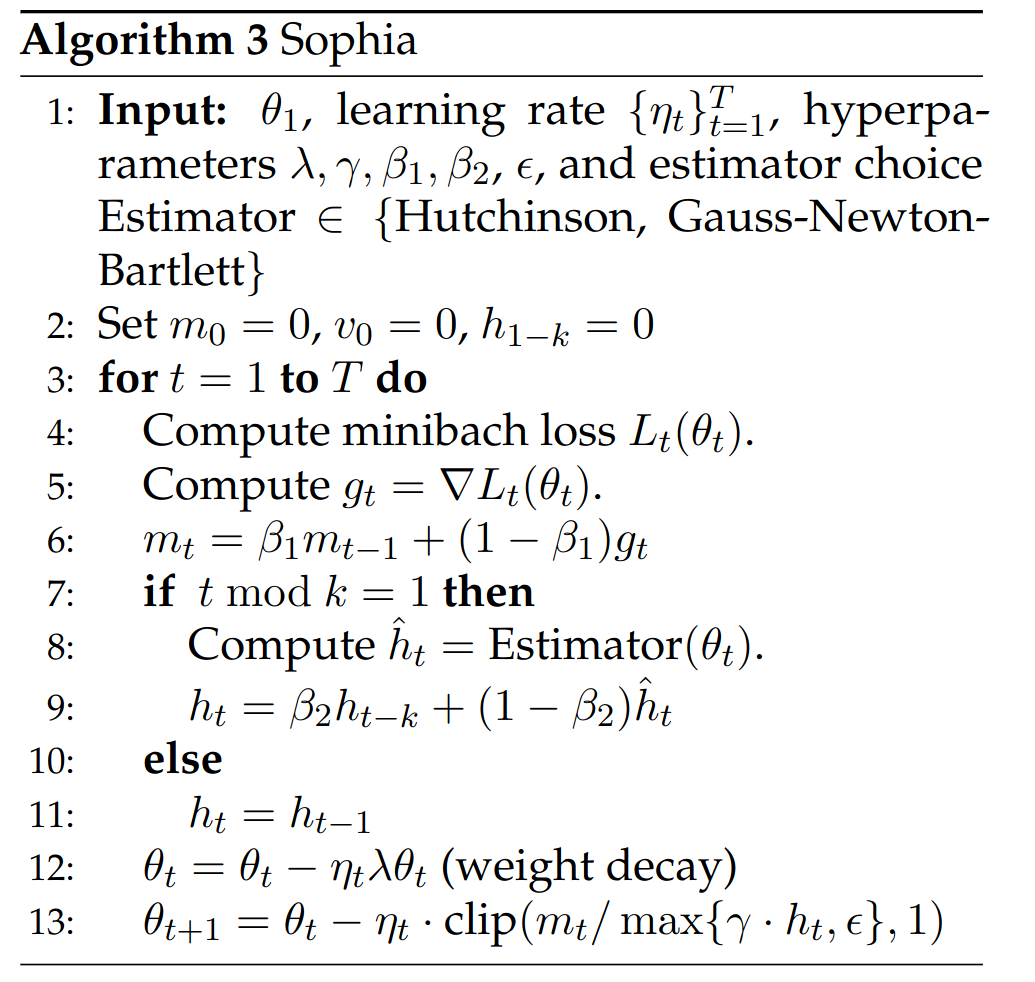
\includegraphics[width=6.5cm]{figures/sophia_algo.png}
        	    \caption*{Claude Shannon}
        	\end{figure}
		\end{column}
	\end{columns}
\end{frame}

\begin{frame}{Defining 2x faster }
\begin{columns}[c] % The "c" option specifies centered vertical alignment while the "t" option is used for top vertical alignment
		\begin{column}{0.45\textwidth} % Left column width
			\begin{figure}
				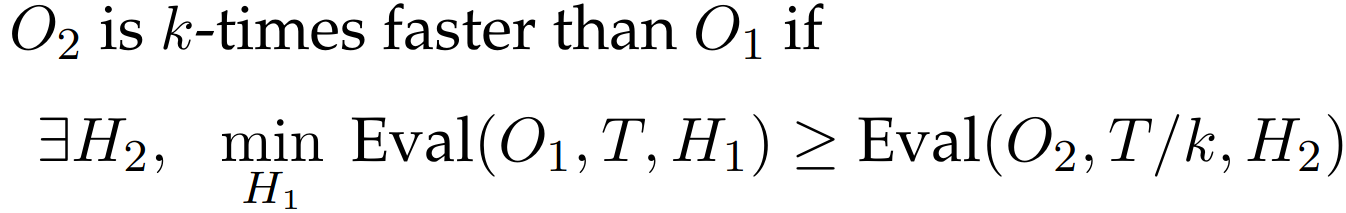
\includegraphics[width=8cm]{figures/2xfaster.png}
			\end{figure}
		\end{column}
		\begin{column}{0.55\textwidth} % Right column width
        	\begin{figure}
        	    \centering
                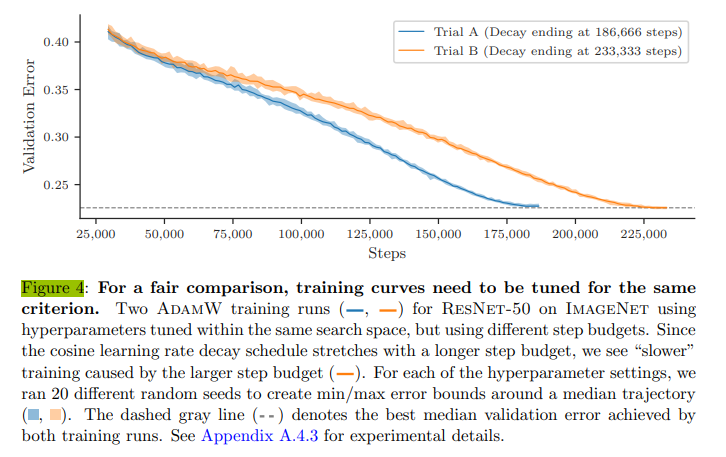
\includegraphics[width=7.5cm]{figures/figure4_dahl_et_al.PNG}
        	\end{figure}
		\end{column}
	\end{columns}
\end{frame}


%------------------------------------------------

\begin{frame}{Lion: EvoLved Sign Momentum}
	\framesubtitle{Why not breed your dream optimizer via evolution}
	\vspace{-1em}
\begin{columns}[c] % The "c" option specifies centered vertical alignment while the "t" option is used for top vertical alignment
		\begin{column}{0.45\textwidth} % Left column width
			\begin{itemize}
					\item 
				\item performs better on larger batch sizes
			\end{itemize}
		\end{column}
		\begin{column}{0.55\textwidth} % Right column width
        	\begin{figure}
        	    \centering
                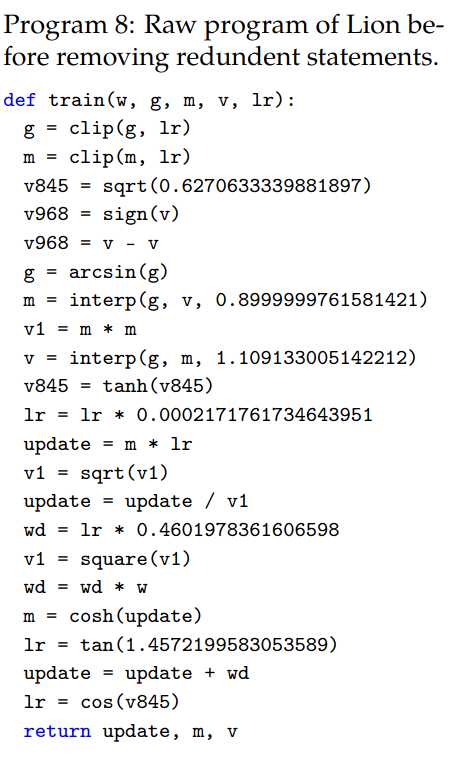
\includegraphics[width=4.4cm]{figures/raw_lion.png}
        	\end{figure}
		\end{column}
	\end{columns}
\end{frame}

\subsection{Evidence Lower Bound \& Entropy Coding}


\begin{frame}{Entropy Coding}
	 \begin{columns}[c] % The "c" option specifies centered vertical alignment while the "t" option is used for top vertical alignment
		\begin{column}{0.45\textwidth} % Left column width
			\begin{center}
			Shannon's source coding theorem:\\
			"The Entropy $H(p)$ is a lower bound for lossless data compression":
			\end{center}
			\begin{align*}
        	H(p) =& - \sum_{\mathbf{X}\in \mathcal{X}} \textcolor{red}{p(\mathbf{X})} \log_2 \textcolor{red}{p(\mathbf{X})}\\
			\\\vspace{1em}\\
        H(p_{\text{data}}, p_{\text{model}}) =& - \sum_{\mathbf{X}\in \mathcal{X}} p_{\text{data}}(\mathbf{X}) \log_2 p_{\text{model}}(\mathbf{X}) \\
        =& ~ H(p_{\text{data}}) + \underbrace{D_{KL}(p_{\text{data}} ||~ p_{\text{model}})}_{\text{modeling gap}}
			\end{align*}
		\end{column}
		\begin{column}{0.55\textwidth} % Right column width
        	\begin{figure}
        	    \centering
                % \includegraphics[width=4.5cm]{figures/shannon.jpg}
        	    \caption*{Claude Shannon}
        	\end{figure}
		\end{column}
	\end{columns}
\end{frame}

\begin{frame}{A Latent Variable Model for $p_{\text{model}}$}
		\begin{figure}[ht]
        \centering
		% \includegraphics[width=8cm]{figures/LVM.png}
        \caption{Graphical representation of a Latent Variable Model. $\mathbf{Z}$ is called the latent variable and  $X_i$ the target message.}
        \label{fig:LVM}
    \end{figure}
	\begin{align}
        p(\mathbf{X}, \mathbf{Z})&= \prod_{i=1}^{n}p(X_i\mid\mathbf{Z})p(\mathbf{Z}) \\
        p(\mathbf{X}) &=\textcolor{red}{\int_{\mathbf{Z} \in \mathcal{Z}}} p(\mathbf{X}, \mathbf{Z}) \; \textcolor{red}{d\mathbf{Z}}
	\end{align}
\end{frame}

 \begin{frame}
	\frametitle{A tractable LVM: VAEs minimizing a NELBO}
	Variational approximation of the true posterior: $\underbrace{q_{\phi}(\mathbf{Z} \mid \mathbf{X})}_{\text{encoder model}}$
    \begin{align*}
       h(\mathbf{X}) =& -\log p(\mathbf{X}) \le -\text{ELBO}\\
        =&~\mathbb{E}_{\mathbf{Z} \sim q_\phi(\mathbf{Z}\mid \mathbf{X})} [- \log  p_\psi(\mathbf{X}  \mid \mathbf{Z})] + D_{KL}(q_\phi(\mathbf{Z}\mid \mathbf{X}) \mid\mid p(\mathbf{Z}))\\
        =&~ \mathbb{E}_{\mathbf{Z} \sim q_\phi(\mathbf{Z}\mid \mathbf{X})} [- \log  p_\psi(\mathbf{X}  \mid \mathbf{Z}) - \log  p(\mathbf{Z}) + \log q_\phi(\mathbf{Z}\mid \mathbf{X})] 
    \end{align*}
	$\Longrightarrow$ the NELBO is an upper bound for the bit rate in lossless data compression
\end{frame}

%------------------------------------------------


%------------------------------------------------


\begin{frame}[plain] % The optional argument 'plain' hides the headline and footline
	\begin{center}
		{\Huge Summary: What is the empirical bit rate for data compression in MRI?}
		
		\bigskip\bigskip % Vertical whitespace
		
	\end{center}
\end{frame}
%------------------------------------------------

 \begin{frame}
 \frametitle{negative ELBOW}
    \begin{figure}
        \begin{center}
        % \includegraphics[width=7cm]{/mnt/Bachelorarbeit/LOLs/negative_elbow.jpg}
        \end{center}
    \end{figure}
\end{frame}

%------------------------------------------------


\end{document} 